\documentclass[10pt]{beamer}

\usetheme[progressbar=frametitle]{metropolis}
\usepackage{appendixnumberbeamer}

\usepackage{booktabs}
\usepackage[scale=2]{ccicons}

\usepackage{pgfplots}
\usepgfplotslibrary{dateplot}

\usepackage{xspace}
\newcommand{\themename}{\textbf{\textsc{metropolis}}\xspace}

\usepackage{booktabs}

\title{\vspace*{1.5cm}Dynamic Adaptive Streaming over HTTP}
\subtitle{DASH}
\date{\vspace*{1cm}\centering 19 September 2017}
\author{Luca Mazzon 1151499 \hfill Luca Vallerini 1110975}
\institute{\centering Computer Networks - Academic Year 2016/2017}
\titlegraphic{
\includegraphics[height=1.5cm]{logos/sublogo_3}\hfill
\includegraphics[height=1.5cm]{logos/unipd_logo}}

\begin{document}

\maketitle

\setbeamertemplate{frame footer}{Luca Mazzon, Luca Vallerini - Computer Networks - A.Y. 2016/2017}

\begin{frame}[fragile]{Contents}
We organized our chapter in two parts:
\begin{enumerate}
\item MPEG-DASH protocol breakdown and design principles, with references to other protocols
\item Analysis of the Adaptive Bit Rate algorithm SARA
\end{enumerate}
\end{frame}

\begin{frame}[fragile]{What is DASH}
Dynamic Adaptive Streaming over HTTP (DASH) is a video streaming protocol which is capable of dynamically adapt to the conditions of the system in order to provide seamless video playback.
\vfill
Different protocols with the same conceptual level:
\begin{itemize}
\item A video is taken from a source and it's encoded with different bitrates;
\item Encoded videos are hosted on HTTP servers and fragmented;
\item A client progressively downloads and plays back the segments choosing dynamically the best bitrate for the network condition.
\end{itemize}
\end{frame}

\begin{frame}[fragile]{Why is DASH important?}
Cisco Visual Networking Index Mobile Data Forecast for 2021 expect that video data will account for 78\% of the mobile data traffic (more than 38 Exabytes per month).

\centering
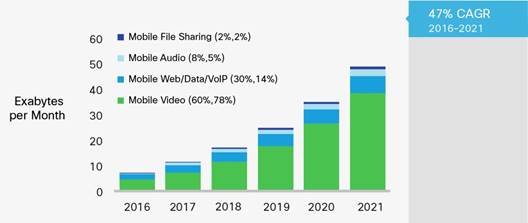
\includegraphics[width=0.5\textwidth]{img/Cisco}

An increase in demand and in quality expectation from users require appropriate advanced technologies like DASH.
\end{frame}

\begin{frame}[fragile]{Different protocols, same idea}
\begin{table}[]
\centering
\label{my-label}
\begin{tabular}{@{}ll@{}}
\toprule
Company   & Protocol                                            \\ \midrule
MPEG      & MPEG-DASH (ISO/IEC23009)                            \\
3GPP      & Adaptive HTTP Streaming (AHS) (TS 26.233 ...)       \\
Apple     & HTTP Live Streaming (Internet-Draft, Informational) \\ 
Microsoft & Smooth Streaming Protocol (MS-SSTR)                 \\
Adobe     & HTTP Dynamic Streaming                              \\ \bottomrule
\end{tabular}
\end{table}
\end{frame}

\begin{frame}[fragile]{MPEG-DASH Data Model}
Three core elements:
\begin{itemize}
\item \textbf{Media Presentation Description}: XML formatted file which describes the Media Presentation, which is a bounded or unbounded list of HTTP URLs to the Segments which compose the video to be streamed;
\item \textbf{Segment}: content response of an HTTP GET or partial HTTP GET. A Segment can contain both media data and metadata.
\item \textbf{Period}: media content period during which the encoded versions of the media are consistent.
\end{itemize}
The content within a Period is arranged in an \textbf{Adaptation Set}, which contains different \textbf{Representations} of the media. Representations are deliverable encoded versions of one or several media content components, such as different resolutions, subtitles, languages and captions. Representations are then divided into Segments.
\end{frame}

\begin{frame}[fragile]{MPEG-DASH MPD structure and streaming Schema}
\begin{columns}
		\column{0.5\linewidth}
        	\centering
            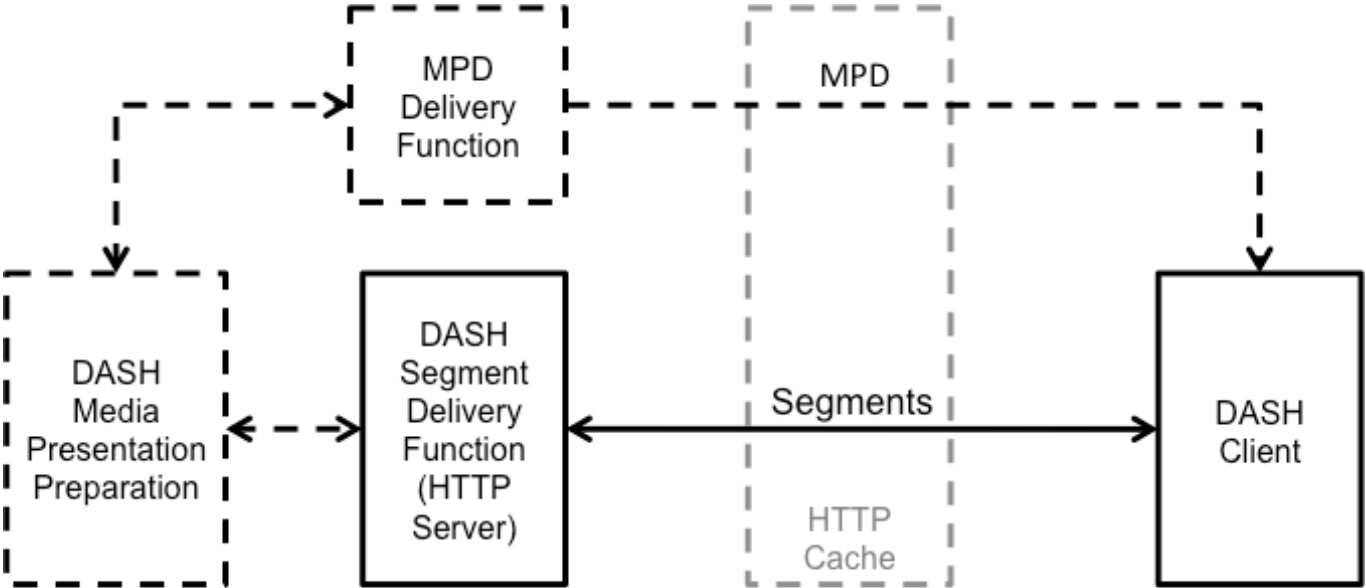
\includegraphics[width=\textwidth]{img/DASH_schema}
            \vspace*{0.5cm}
            \raggedright The client first requests the MPD and then progressively requests the Segments to be played back, until the broadcast ends or the user interrupts the process. The MPD is periodically refreshed to update the list of URLs.
        \column{0.5\linewidth}
        	\centering
            MPD Structure\vspace*{0.25cm}
            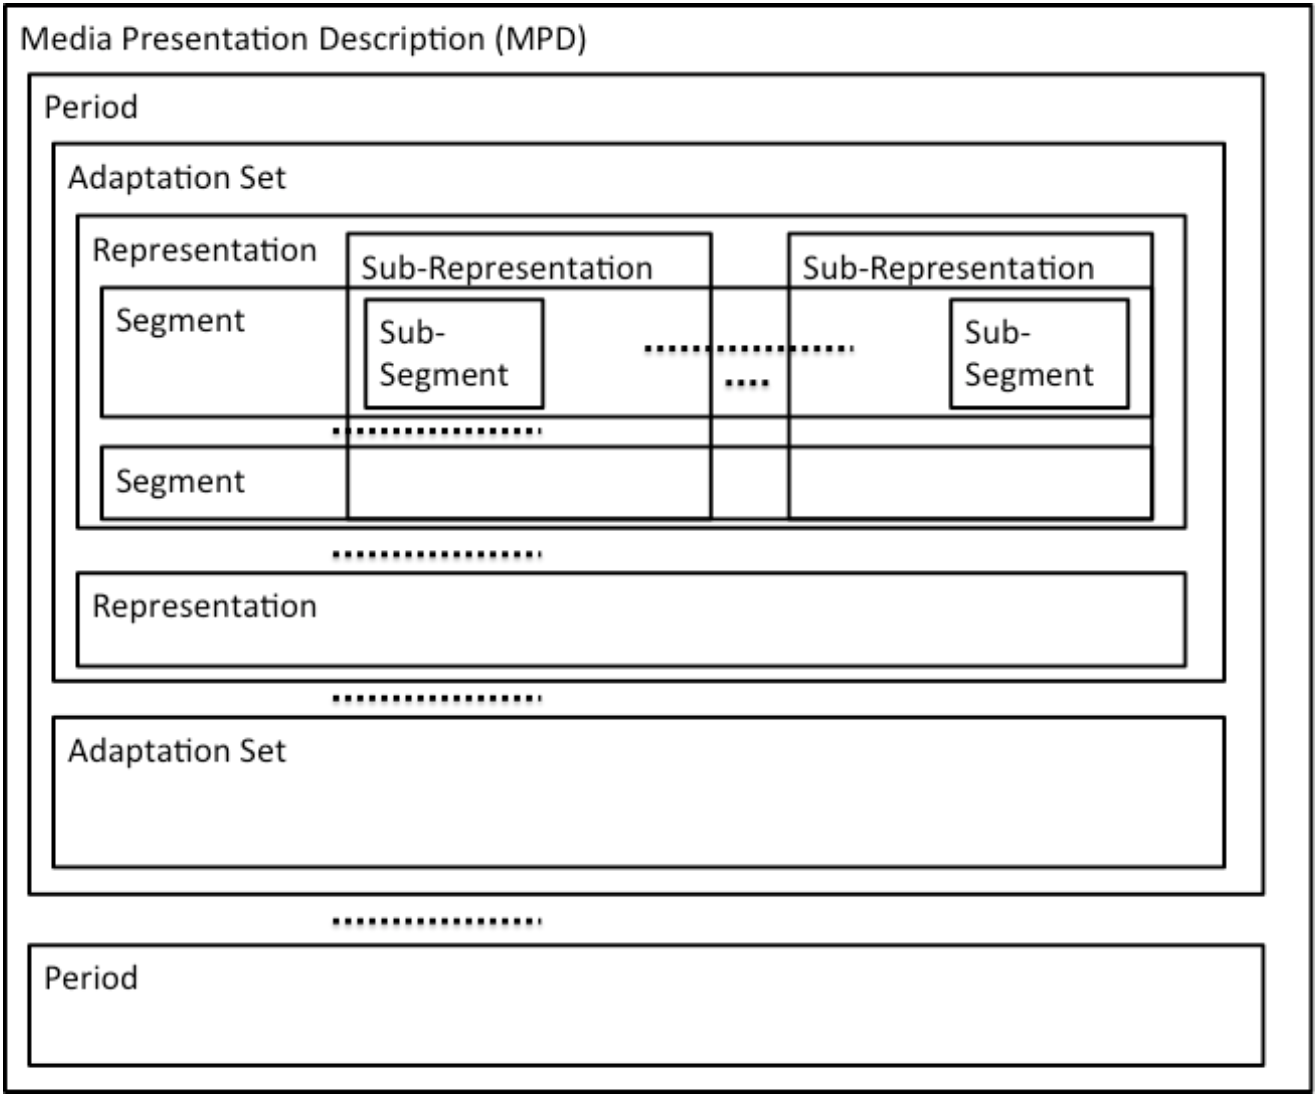
\includegraphics[width=\textwidth]{img/MPD}
\end{columns}
\end{frame}

\begin{frame}[fragile]{Why HTTP?}
\begin{columns}
		\column{0.5\linewidth}
        	\centering
            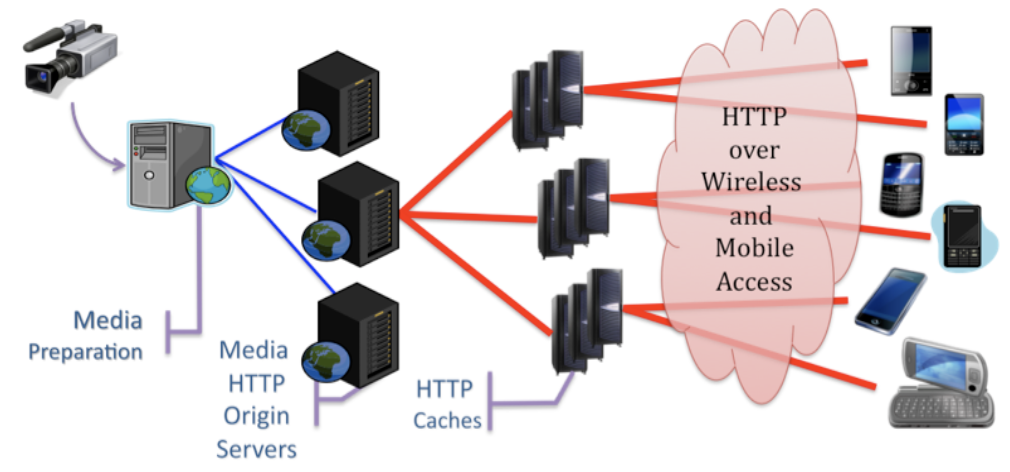
\includegraphics[width=\textwidth]{img/architecture}
            \vspace*{0.25cm}
            \raggedright HTTP is the most used protocol for content delivery and communication over WWW, so preexisting CDNs can be exploited and there aren't any firewall issues.
        \column{0.5\linewidth}
        	\begin{enumerate}
            \item Offload the central server with peripheral servers;
            \item Faster media access with HTTP Caches;
            \item Stateless connection: no extra space on server and data overhead for maintaining state, the client can decide autonomously initial bitrate and variations without having to negotiate with the server (faster adaptation).
            \end{enumerate}
\end{columns}
\end{frame}

\begin{frame}[fragile]{ABR algorithm and SARA}
Adaptive Bit Rate (ABR) algorithms are designed with three goals in mind:
\begin{itemize}
\item Maximize efficiency
\item Minimize re-buffering
\item Stability
\end{itemize}
\vfill
Segment Aware Rate Adaptation (SARA) proposes to enhance the MPD file with the size of each segment and then estimates the throughput based also on this information.
\end{frame}

\begin{frame}[fragile]{SARA: throughput estimate}
To better estimate the throughput SARA uses the Harmonic mean. For a generic segment $i$ a weight $w_i$ proportional to the segment size is assigned. Call $d_i$ the download rate of segment $i$. Then, the weighted harmonic mean download rate of the first $n$ segments is
\[
H_n=\frac{\sum_{i=1}^n w_i}{\sum_{i=1}^n \frac{w_i}{d_i}}
\]

SARA can then estimate the download time of the next segment as $\hat{d}_{n+1}=w_{n+1}/H_n$.
\end{frame}

\begin{frame}[fragile]{SARA: buffer}
The buffer $B$ stores each downloaded segment and feeds the video player with them.

\centering
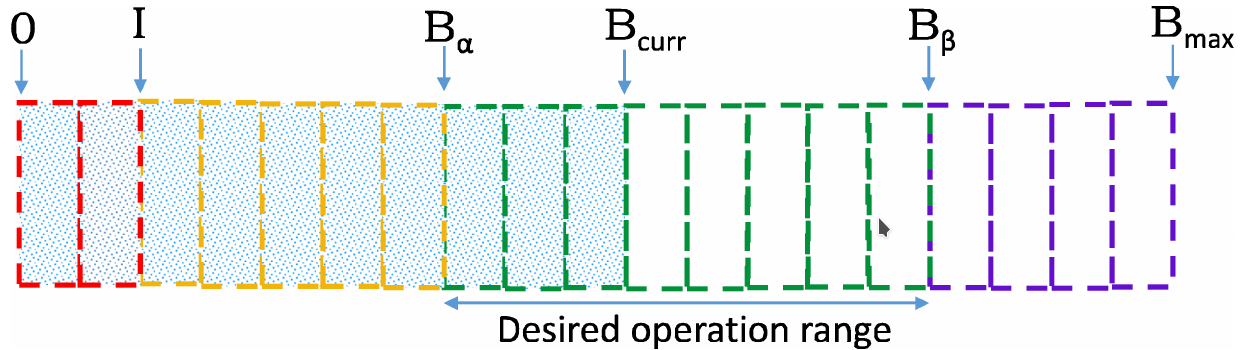
\includegraphics[width=0.5\textwidth]{img/sara_buffer_thresholds}

SARA identifies four thresholds ($I$, $B_{\alpha}$, $B_{\beta}$ and $B_{max}$) and it uses them to decide which representation to download for the next segment. The idea is to keep the buffer in the $[B_\alpha, B_\beta]$ range.
\end{frame}

\begin{frame}[fragile]{SARA: algorithm}
	\begin{columns}
		\column{0.5\linewidth}
        	\centering
            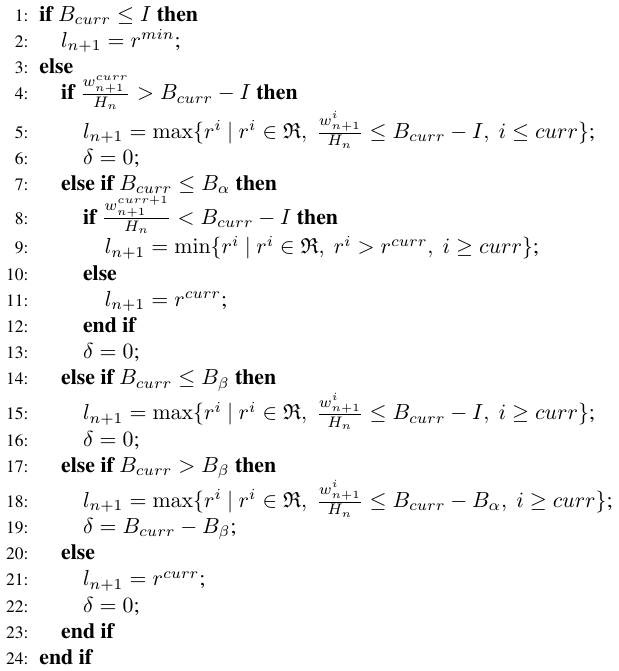
\includegraphics[width=\textwidth]{img/sara_algorithm}
        \column{0.5\linewidth}
        	\textbf{Fast Start} ($B_{curr}\leq I$) The algorithm selects the lowest bit rate.
            
            \textbf{Additive Increase} ($I<B_{curr}\leq B_{\alpha}$) The algorithm starts to increase the bit rate in small steps.
            
            \textbf{Aggressive Switching} ($B_\alpha < B_{curr} \leq B_\beta$) The algorithm selects the most suitable bit rate.
            
            \textbf{Delayed Download} ($B_\beta < B_{curr}\leq B_{max}$) Same as \textit{Aggressive Switching} but the request of the next segment is delayed.
\end{columns}
\end{frame}

\begin{frame}[fragile]{SARA: performance}
	\begin{columns}
		\column{0.5\linewidth}
        	\centering
            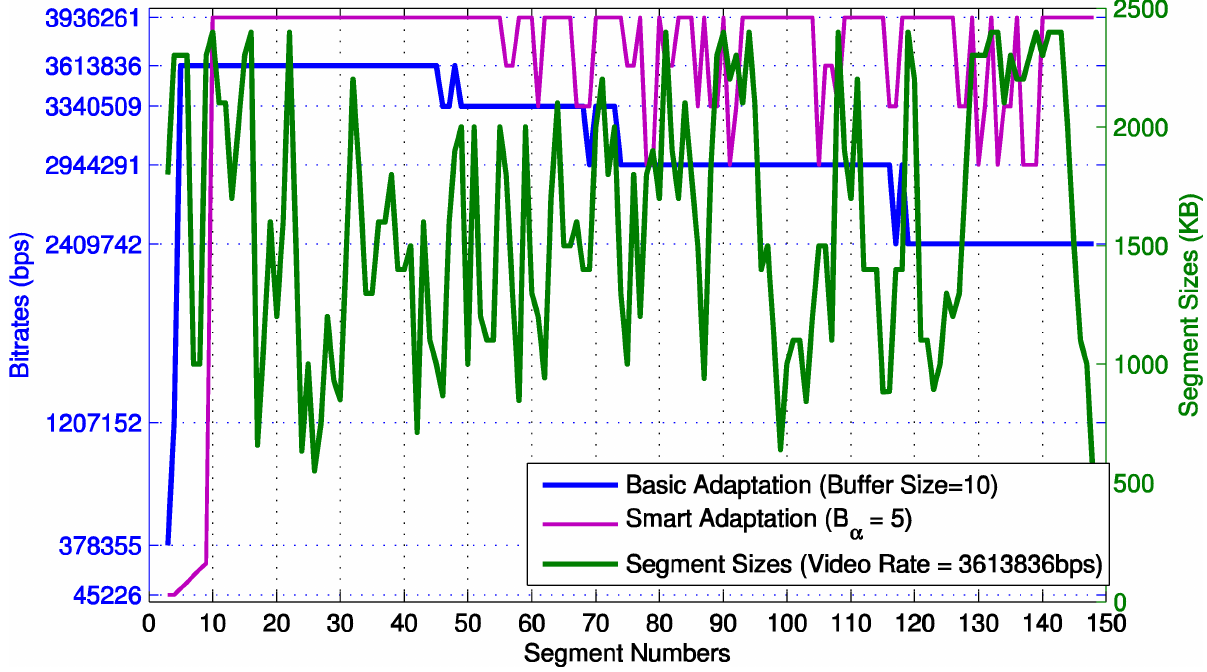
\includegraphics[width=\textwidth]{img/sara_basic_segment}
            \vspace*{0.5cm}
            
            \raggedright Three examples that compares SARA with a basic adaptation algorithm with different bandwidths: $1$ Mbps (above), $4$ Mbps (right, top) and $8$ Mbps (right, bottom).
        \column{0.5\linewidth}
        	\centering
            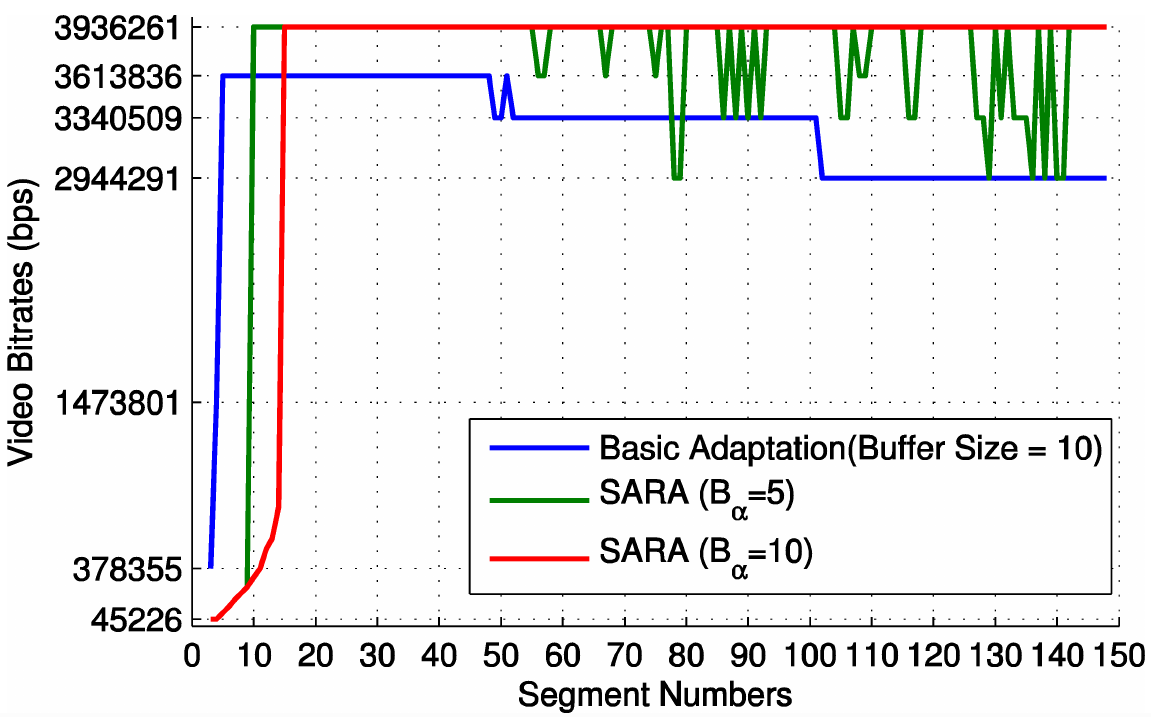
\includegraphics[width=\textwidth]{img/sara_basic_4m}
            \vspace*{0.5cm}
            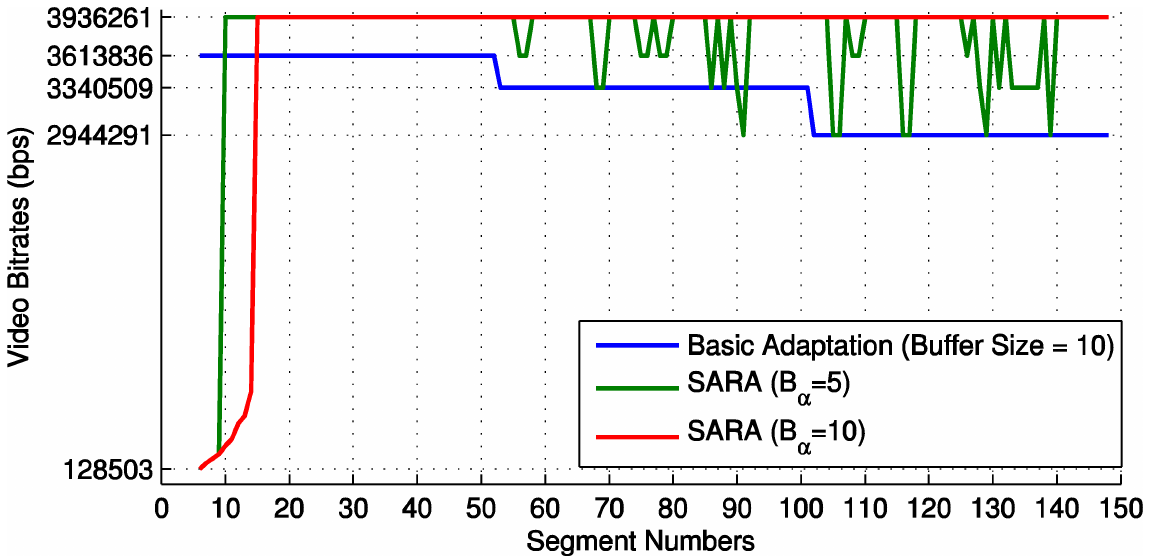
\includegraphics[width=\textwidth]{img/sara_basic_8m}
\end{columns}
\end{frame}

\begin{frame}[fragile]{}
Thank you for your attention.
\end{frame}

\end{document}


